% !TeX program = lualatex
% !BIB program = bibtex
% !TeX encoding = utf8

\documentclass[a4paper]{jpconf}
\usepackage{graphicx}
\usepackage{tikz}
\usepackage{markdown}
\usetikzlibrary{decorations.pathreplacing}

\bibliographystyle{iopart-num}

\begin{document}
\title{A hybrid deep learning approach to vertexing}

\author{
   Rui Fang\textsuperscript{1},
   Henry F Schreiner\textsuperscript{1,2},
   Mike D Sokoloff\textsuperscript{1},
   Constantin Weisser\textsuperscript{3} and
   Mike Williams\textsuperscript{3}
}

\address{
    \textsuperscript{1} University of Cincinnati, Cincinnati, OH, United States
}
\address{
    \textsuperscript{2} Princeton University, Princeton, NJ, United States
}
\address{
    \textsuperscript{3} Massachusetts Institute of Technology, Cambridge, MA, United States
}

\ead{hschrein@cern.ch, others}

\begin{abstract}
In the transition to Run 3 in 2021, LHCb will undergo a major luminosity upgrade, going from 1.1 to 5.6 expected visible Primary Vertices (PVs) per event, and will adopt a purely software trigger. This has fueled increased interest in alternative highly-parallel and GPU friendly algorithms for tracking and reconstruction. We will present a novel prototype algorithm for vertexing in the LHCb upgrade conditions.
We use a custom kernel to transform the sparse 3D space of hits and tracks into a dense 1D dataset, and then apply Deep Learning techniques to find PV locations. By training networks on our kernels using several Convolutional Neural Network layers, we have achieved better than 90\% efficiency with no more than 0.2 False Positives (FPs) per event. Beyond its physics performance, this algorithm also provides a rich collection of possibilities for visualization and study of 1D convolutional networks. We will discuss the design, performance, and future potential areas of improvement and study, such as possible ways to recover the full 3D vertex information.
\end{abstract}


\section{Introduction}

% TODO: Write this up

The LHCb detector is facing a major upgrade in luminosity in Run 3 in 2021. In each event, the Poisson average expected for the visible Primary Vertices (PVs) will go from 1.1 to 5.6. In addition, the hardware level-0 trigger is being removed in favor of a purely software trigger running at 30 MHz \cite{CERN-LHCC-2014-016}. Work is ongoing to find new algorithms to support the upgrade era software for LHCb.

The current algorithm for finding vertices is TODO.

An alternate method is proposed here for finding vertices from tracks or hits using machine learning techniques. The algorithm starts with tracks containing location, direction, and covariance matrix information. The tracks in 3D space are converted to a 1D binned ``kernel'' through a process described below. Peaks in this kernel are closely related to the z positions of the primary verticies. We use a series of 1D convolutional layers to predict the PV locations from this kernel. The output probabilities from the neural network are converted to a list of PV candidate z-locations using a simple peak finding algorithm. Using this procedure we have surpassed 90\% efficency with less than 0.2 False Positives (FPs) per event.

A toy simulation of the LHCb detector has been developed to test this algorithm. The design of the algorithm and the toy that is was tested with follows.

\section{Kernel Generation}

The algorithm we are about to describe applies to tracks; though even a simple and inaccurate procedure is sufficient. Our toy simulation generates tracks from PVs and SVs, and we using a simple intersection procedure to produces hits in the Vertex Locater (VELO) according to a simple model of the detector (REF). The hits in the detector are then fed into a ``prototracking'' algorithm, which is a simple but sufficient tracking system 

In order to provide a simple, dense representation for the machine learning algorithm to use, the tracks are transformed into a dense representation using a ``kernel'' procedure. 

\section{Network Design}

The following 

\begin{figure}
   \centering
   \newcounter{layer}
\setcounter{layer}{0}
\def\wid{3.7}

\begin{tikzpicture}[
    scale=.77,
    every node/.style={scale=.77}]

% Layer 1
\begin{scope}[xshift=\thelayer*\wid cm]
\node at (0,0) {Inputs};
\foreach \i [count=\xi] in {1,2,3,$\cdots$,25,26,$\cdots$,3998,3999,4000} {
    \node at(0, -\xi/2) [draw, minimum width = 1cm, minimum height = .5cm] {\i};
}

\draw [decorate,decoration={brace,amplitude=10pt}] (.5,-.25) -- (.5,-2.75);
\draw [-latex] (.6, -2.75) -- (.6, -3.2);
\draw [-latex] (.9, -1.5) -- (\wid - 1, -1.5);
\begin{scope}[xshift=.5cm, yshift=-3.5cm]
\node at (0, 0) [right] {Convolution};
\node at (0,  -.6) [right] {Width:};
\node at (.5, -1) [right] {25};
\node at (0, -1.4) [right] {Channels:};
\node at (.5, -1.8) [right] {$1\rightarrow25$};
\end{scope}
\end{scope}
\stepcounter{layer}

% Layer 2
\begin{scope}[xshift=\thelayer*\wid cm]
\node at (0,0) {25 Channels};
% Backing
\foreach \i in {.5,.45,.4,.35,.3,.25,.2,.15,.1,.05} {
	\begin{scope}[xshift=-.5cm-\i cm, yshift=-.25cm -\i cm]
	\path[fill=white] (0,0) rectangle (1,-5);
	\draw [opacity=1-\i*2 + .05, ystep=.5] (0,0) grid (1,-5);
	\end{scope}
}
\foreach \i [count=\xi] in {1,2,3,$\cdots$,15,16,$\cdots$,3998,3999,4000} {
	\node at(0, -\xi/2) [draw, fill=white, minimum width = 1cm, minimum height = .5cm] {\i};
}

\draw [decorate,decoration={brace,amplitude=10pt}] (.5,-.25) -- (.5,-2.75);
\draw [-latex] (.6, -2.75) -- (.6, -3.2);
\draw [-latex] (.9, -1.5) -- (\wid - 1, -1.5);
\begin{scope}[xshift=.5cm, yshift=-3.5cm]
\node at (0, 0) [right] {Convolution};
\node at (0,  -.6) [right] {Width:};
\node at (.5, -1) [right] {15};
\node at (0, -1.4) [right] {Channels:};
\node at (.5, -1.8) [right] {$25\rightarrow25$};
\end{scope}
\end{scope}
\stepcounter{layer}

% Layer 3
\begin{scope}[xshift=\thelayer*\wid cm]
\node at (0,0) {25 Channels};
% Backing
\foreach \i in {.5,.45,.4,.35,.3,.25,.2,.15,.1,.05} {
	\begin{scope}[xshift=-.5cm-\i cm, yshift=-.25cm -\i cm]
	\path[fill=white] (0,0) rectangle (1,-5);
	\draw [opacity=1-\i*2 + .05, ystep=.5] (0,0) grid (1,-5);
	\end{scope}
}
\foreach \i [count=\xi] in {1,2,3,$\cdots$,15,16,$\cdots$,3998,3999,4000} {
	\node at(0, -\xi/2) [draw, fill=white, minimum width = 1cm, minimum height = .5cm] {\i};
}

\draw [decorate,decoration={brace,amplitude=10pt}] (.5,-.25) -- (.5,-2.75);
\draw [-latex] (.6, -2.75) -- (.6, -3.2);
\draw [-latex] (.9, -1.5) -- (\wid - 1, -1.5);
\begin{scope}[xshift=.5cm, yshift=-3.5cm]
\node at (0, 0) [right] {Convolution};
\node at (0,  -.6) [right] {Width:};
\node at (.5, -1) [right] {15};
\node at (0, -1.4) [right] {Channels:};
\node at (.5, -1.8) [right] {$25\rightarrow25$};
\end{scope}
\end{scope}
\stepcounter{layer}

% Layer 4
\begin{scope}[xshift=\thelayer*\wid cm]
\node at (0,0) {25 Channels};
% Backing
\foreach \i in {.5,.45,.4,.35,.3,.25,.2,.15,.1,.05} {
	\begin{scope}[xshift=-.5cm-\i cm, yshift=-.25cm -\i cm]
	\path[fill=white] (0,0) rectangle (1,-5);
	\draw [opacity=1-\i*2 + .05, ystep=.5] (0,0) grid (1,-5);
	\end{scope}
}
\foreach \i [count=\xi] in {1,2,3,4,5,6,$\cdots$,3998,3999,4000} {
	\node at(0, -\xi/2) [draw, fill=white, minimum width = 1cm, minimum height = .5cm] {\i};
}

\draw [decorate,decoration={brace,amplitude=10pt}] (.5,-.25) -- (.5,-2.75);
\draw [-latex] (.6, -2.75) -- (.6, -3.2);
\draw [-latex] (.9, -1.5) -- (\wid - 1, -1.5);
\begin{scope}[xshift=.5cm, yshift=-3.5cm]
\node at (0, 0) [right] {Convolution};
\node at (0,  -.6) [right] {Width:};
\node at (.5, -1) [right] {5};
\node at (0, -1.4) [right] {Channels:};
\node at (.5, -1.8) [right] {$25\rightarrow1$};
\end{scope}
\end{scope}
\stepcounter{layer}

% Layer 5
\begin{scope}[xshift=\thelayer*\wid cm - .5 cm]
\node at (0,0) {1 Channel};
% Backing
%\foreach \i in {.4,.3,.2,.1} {
%\begin{scope}[xshift=-.5cm-\i cm, yshift=-.25cm -\i cm]
%\path[fill=white] (0,0) rectangle (1,-5);
%\draw [opacity=1-\i*2, ystep=.5] (0,0) grid (1,-5);
%\end{scope}
%}
\foreach \i [count=\xi] in {1,2,3,$\cdots$,91,92,$\cdots$,3998,3999,4000} {
	\node at(0, -\xi/2) [draw, fill=white, minimum width = 1cm, minimum height = .5cm] {\i};
}

\draw [decorate,decoration={brace,amplitude=10pt}] (.5,-.25) -- (.5,-2.75);
\draw [-latex] (.6, -2.75) -- (.6, -3.2);
\draw [-latex] (.9, -1.5) -- (\wid - 1, -1.5);
\begin{scope}[xshift=.5cm, yshift=-3.5cm]
\node at (0, 0) [right] {Convolution};
\node at (0,  -.6) [right] {Width:};
\node at (.5, -1) [right] {91};
\node at (0, -1.4) [right] {Channels:};
\node at (.5, -1.8) [right] {$1\rightarrow1$};
\end{scope}
\end{scope}
\stepcounter{layer}

% Layer Output
\begin{scope}[xshift=\thelayer*\wid cm - 1 cm]
\node at (0,0) {Output};
\foreach \i [count=\xi] in {1,2,3,4,5,$\cdots$,3997,3998,3999,4000} {
	\node at(0, -\xi/2) [draw, fill=white, minimum width = 1cm, minimum height = .5cm] {\i};
}
\end{scope}
\stepcounter{layer}

\begin{scope}[xshift=-.5cm, yshift=-7.5cm]

% Loop as needed
\foreach \i in {\wid * 0.5,\wid * 1.5, \wid * 2.5, \wid * 3.5} {
	\begin{scope}[xshift=\i cm]
	\draw [step=.25] (-1.2, .05) grid (1.2, -.05);
	\draw [step=.25] (-.05, -.2) grid (.05, 1.4);
	\draw [black, latex-latex] (-1.3, 0) node[above] {-x} -- (1.3, 0) node[above] {x};
	\draw [black, latex-latex] (0, -.3)  -- (0, 1.3) node[left] {y};
	\draw [thick, black](-1.3, -.1) -- (0, 0) -- (1.3,1.3);
	\node at (0, -.6) {Leaky relu};
	\end{scope}
}

\begin{scope}[xshift=\wid * 4.5 cm - .25 cm]
\draw [step=.25] (-1.2, .05) grid (1.2, -.05);
\draw [step=.25] (-.05, -.2) grid (.05, 1.4);
\draw [black, latex-latex] (-1.3, 0) node[above] {-x} -- (1.3, 0) node[above] {x};
\draw [black, latex-latex] (0, -.3)  -- (0, 1.3) node[left] {y};
\draw [thick, black, smooth]  plot coordinates {
	(-1.5, 0)
	(0, .25)
	(1.3, 1.3)};
\node at (0, -.6) {Softplus};
\end{scope}

\end{scope}

\end{tikzpicture}
   \caption{The final network architecture used in TODO.}
   \label{fig:nnarch}
\end{figure}

\begin{figure}
  \centering
  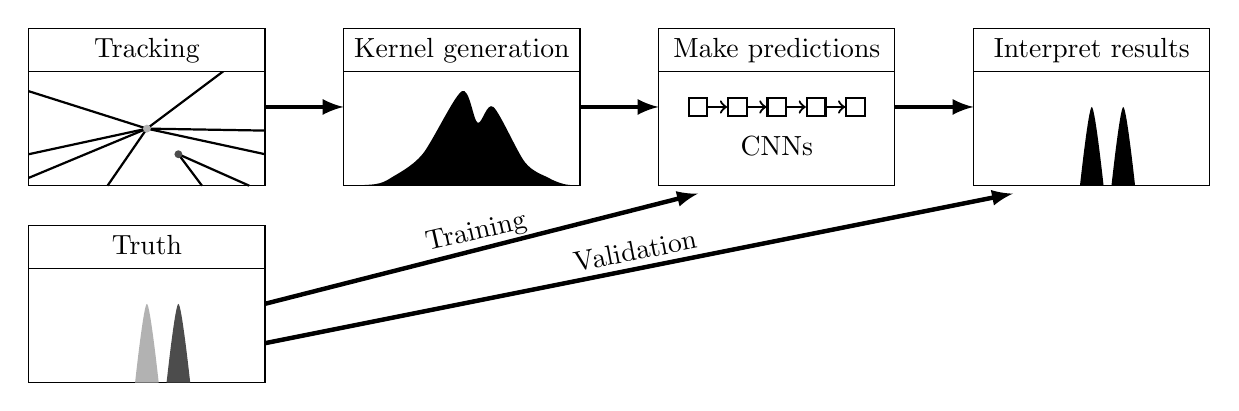
\begin{tikzpicture}[
    scale=1,
    belowbox/.style={draw},
    topbox/.style={draw, fill=white},
    texttop/.style={below},
    track/.style={thick},
    minibox/.style={draw, thick, minimum width=.1cm, minimum height=.1cm},
    miniarr/.style={->, thick},
    conn/.style={-latex, ultra thick}
    ]
    	\begin{scope}
    	    \path [belowbox] (-1.5,-1) rectangle (1.5,.45);
    		\draw [track] (0,-.275) -- (-1.5,-.9);
    		\draw [track] (0,-.275) -- (-1.5,-.6);
    		\draw [track] (0,-.275) -- (-1.5,.2);
    		\draw [track] (0,-.275) -- (1.5,-.3);
    		\draw [track] (0,-.275) -- (1.5,-.6);
    		\draw [track] (0,-.275) -- (1.5,.85);
    		\draw [track] (0,-.275) -- (-.5,-1);
    		\draw [track] (.4, -.6) -- (1.3,-1);
    		\draw [track] (.4, -.6) -- (.7,-1);
    		\path [topbox]  (-1.5,.45) rectangle (1.5,1);
    	    \node at (0,1) [texttop] {Tracking};
            \path [fill=black!30] (0, -.275) circle (.05);
            \path [fill=black!70] (.4, -.6) circle (.05);
    	\end{scope}

    	\begin{scope}[xshift=4cm]
    	    \path [belowbox] (-1.5,-1) rectangle (1.5,.45);
    		\path [fill=black] plot [smooth] coordinates {
    			(-1.5,-1)
    			(-1.1, -.98)
    			(-.9, -.9)
    			(-.5, -.6)
    			(0, .2)
    			(.2, -.2)
    			(.4, 0)
    			(.8, -.7)
    			(1.1, -.9)
    			(1.3, -.98)
    			(1.5,-1)
    		};
    		\path [topbox]  (-1.5,.45) rectangle (1.5,1);
    	    \node at (0,1) [texttop] {Kernel generation};
    	\end{scope}

    	\begin{scope}[xshift=8cm]
    	    \path [belowbox] (-1.5,-1) rectangle (1.5,.45);

            \begin{scope}[yshift=3mm]
        		\node [minibox] (mA) at (-1,-.3) {};
        		\node [minibox] (mB) at (-.5,-.3) {};
        		\node [minibox] (mC) at (0,-.3) {};
        		\node [minibox] (mD) at (.5,-.3) {};
        		\node [minibox] (mE) at (1,-.3) {};
        		\draw [miniarr] (mA) -- (mB);
        		\draw [miniarr] (mB) -- (mC);
        		\draw [miniarr] (mC) -- (mD);
        		\draw [miniarr] (mD) -- (mE);
            \end{scope}

    		\path [topbox]  (-1.5,.45) rectangle (1.5,1);
    	    \node at (0,1) [texttop] {Make predictions};
            \node at (0,-.5) {CNNs};
    	\end{scope}

    	\begin{scope}[xshift=12cm]
    	    \path [belowbox] (-1.5,-1) rectangle (1.5,.45);
    		\path [fill=black] plot [smooth] coordinates {
    		(-.15,-1)
    		(0, 0)
    		(.15,-1)
    		};
    		\path [fill=black] plot [smooth] coordinates {
    		(.25,-1)
    		(.4, 0)
    		(.55,-1)
    		};
    		\path [topbox]  (-1.5,.45) rectangle (1.5,1);
    	    \node at (0,1) [texttop] {Interpret results};
    	\end{scope}

    	\begin{scope}[xshift=0cm, yshift=-2.5cm]
    	    \path [belowbox] (-1.5,-1) rectangle (1.5,.45);
    		\path [fill=black!30] plot [smooth] coordinates {
    		(-.15,-1)
    		(0, 0)
    		(.15,-1)
    		};
    		\path [fill=black!70] plot [smooth] coordinates {
    		(.25,-1)
    		(.4, 0)
    		(.55,-1)
    		};
    		\path [topbox]  (-1.5,.45) rectangle (1.5,1);
    	    \node at (0,1) [texttop] {Truth};
    	\end{scope}

    	\draw [conn] (1.5,0) -- (2.5,0);
    	\draw [conn] (5.5,0) -- (6.5,0);
    	\draw [conn] (9.5,0) -- (10.5,0);
    	\draw [conn] (1.5, -2.5) -- (7, -1.1) node [above=-2.5, midway, rotate=13] {Training};
    	\draw [conn] (1.5, -3) -- (11, -1.1) node [above=-1, midway, rotate=11] {Validation};
\end{tikzpicture}
  \caption{The final network architecture used in TODO.}
  \label{fig:approach}
\end{figure}

\begin{figure}
	\centering
	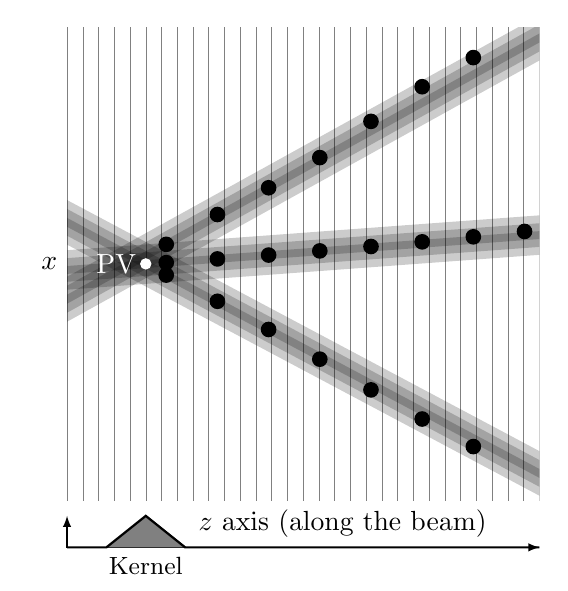
\begin{tikzpicture}[
    hit/.style={inner sep=2pt, fill, circle, black},
    simitrack/.style={shorten >= -6cm, shorten <= -6cm, opacity=.2, line width=.1cm,
        preaction={draw, line width=.3cm, opacity=.2},
        preaction={draw, line width=.5cm, opacity=.2}},
    bluesimitrack/.style={thick, blue,
        preaction={shorten >= -6cm, shorten <= -6cm, draw, opacity=.2, line width=.1cm,
            preaction={draw, blue, line width=.3cm, opacity=.2},
            preaction={draw, blue, line width=.5cm, opacity=.2}}}
        ]

    \path [use as bounding box] (-1.5,-3.8) rectangle (5,3);

    \node at (2.5,-3) [below] {$z$ axis (along the beam)};
    \node at (-1, 0) [left] {$x$};


        \begin{scope}[yshift=-3.6cm]
            \draw [latex-latex] (-1,.4) -- (-1,0) -- (5,0);
            \draw [thick, black, fill=gray]
                (-1,0) -- (-.5,0) -- (0,.4) -- (.5, 0) -- (5,0);
            \node at (0,0) [below] {\small Kernel};
        \end{scope}

    \clip (-1,-3) rectangle (5,3);

    \begin{scope}[xscale=.65, xshift=-.6cm]

        % def f(name, slope, factor):
        %     v = np.arange(1,9)
        %     vv = (v-.5)*slope + .05*np.sin(v*factor)
        %     q = np.linspace(.5, 8, 400)
        %     qq = (q-.5)*slope + .05*np.sin(q*factor)
        %     print(f'% {name} slope={slope} factor={factor}')
        %     for a,b in zip(v,vv):
        %         print(f'\coordinate ({name}{a}) at ({a}, {b:.3});')
        %     print()
        %     return q, qq, v, vv


        % (v-.5)*slope + .05*np.sin(v*factor)
        % A slope=0.4 factor=-5
        \coordinate (A7) at (1, 0.248);
        \coordinate (A6) at (2, 0.627);
        \coordinate (A5) at (3, 0.967);
        \coordinate (A4) at (4, 1.35);
        \coordinate (A3) at (5, 1.81);
        \coordinate (A2) at (6, 2.25);
        \coordinate (A1) at (7, 2.62);

        % B slope=0.06 factor=6
        \coordinate (B8) at (1, 0.016);
        \coordinate (B7) at (2, 0.0632);
        \coordinate (B6) at (3, 0.112);
        \coordinate (B5) at (4, 0.165);
        \coordinate (B4) at (5, 0.221);
        \coordinate (B3) at (6, 0.28);
        \coordinate (B2) at (7, 0.344);
        \coordinate (B1) at (8, 0.412);

        % C slope=-0.35 factor=7
        \coordinate (C7) at (1, -0.142);
        \coordinate (C6) at (2, -0.475);
        \coordinate (C5) at (3, -0.833);
        \coordinate (C4) at (4, -1.21);
        \coordinate (C3) at (5, -1.6);
        \coordinate (C2) at (6, -1.97);
        \coordinate (C1) at (7, -2.32);

    \end{scope}


    \draw[xstep=.2, ystep=10, yshift=-4cm, gray, very thin, use as bounding box] (-1,0) grid (5,8);

    \draw [simitrack] (A5) -- (A7) ;
    \draw [simitrack] (B6) -- (B8) ;
    \draw [simitrack] (C5) -- (C7) ;

    \draw [fill,white] (0,0) circle (.065) node [left] {PV};

    \node [hit] at (A1) {};
    \node [hit] at (A2) {};
    \node [hit] at (A3) {};
    \node [hit] at (A4) {};
    \node [hit] at (A5) {};
    \node [hit] at (A6) {};
    \node [hit] at (A7) {};

    \node [hit] at (B1) {};
    \node [hit] at (B2) {};
    \node [hit] at (B3) {};
    \node [hit] at (B4) {};
    \node [hit] at (B5) {};
    \node [hit] at (B6) {};
    \node [hit] at (B7) {};
    \node [hit] at (B8) {};

    \node [hit] at (C1) {};
    \node [hit] at (C2) {};
    \node [hit] at (C3) {};
    \node [hit] at (C4) {};
    \node [hit] at (C5) {};
    \node [hit] at (C6) {};
    \node [hit] at (C7) {};

\end{tikzpicture}

	\caption{The kernel TODO.}
	\label{fig:kernel}
\end{figure}

\begin{figure}
	\centering
	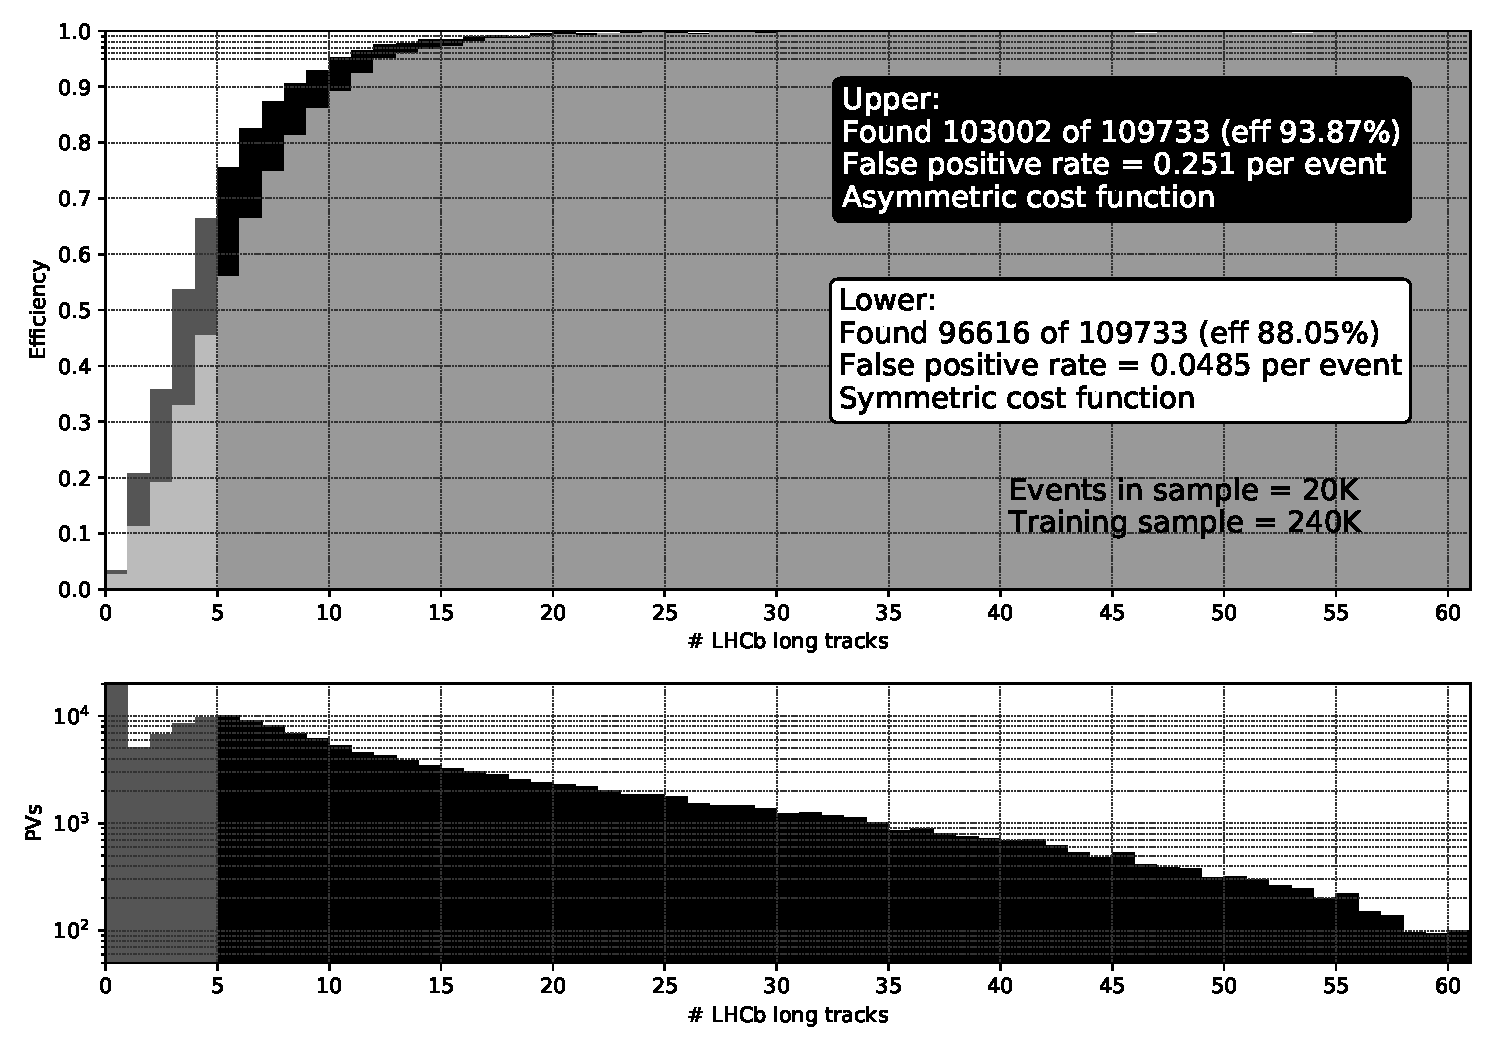
\includegraphics[width=\textwidth]{images/effntrackspaper.pdf}
	\caption{The Results TODO.}
    \label{fig:results}
\end{figure}

\begin{figure}
	\centering
	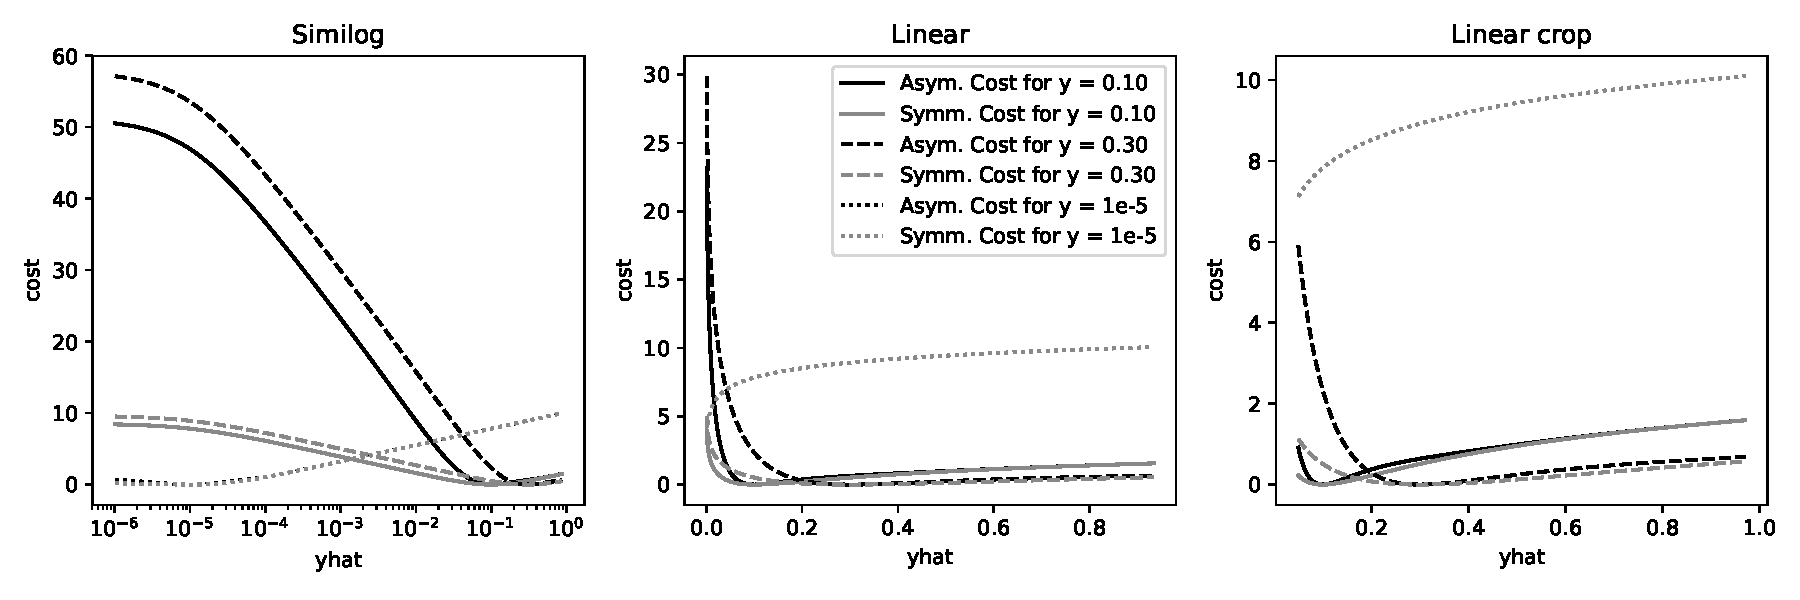
\includegraphics[width=\textwidth]{images/LossPaper.pdf}
	\caption{The Results TODO.}
	\label{fig:loss}
\end{figure}

\begin{figure}
	\centering
	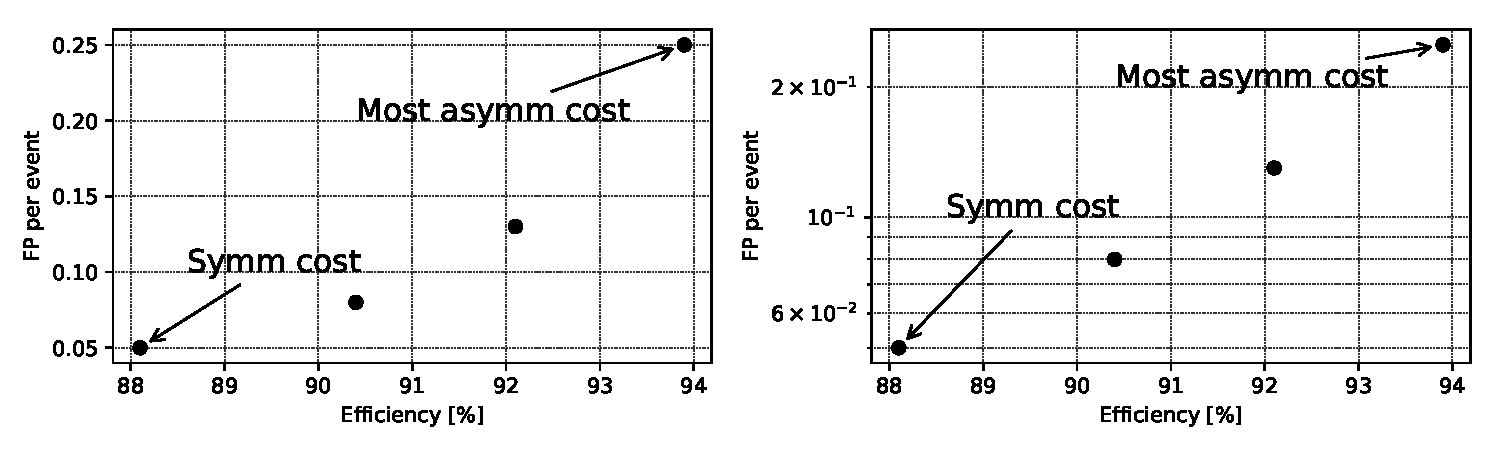
\includegraphics[width=.8\textwidth]{images/EffVsFP2paper.pdf}
	\caption{The Results TODO.}
	\label{fig:efffp}
\end{figure}




\section{Results}

\section{Plans}

\section*{References}

\bibliography{pvfinder}

\end{document}


